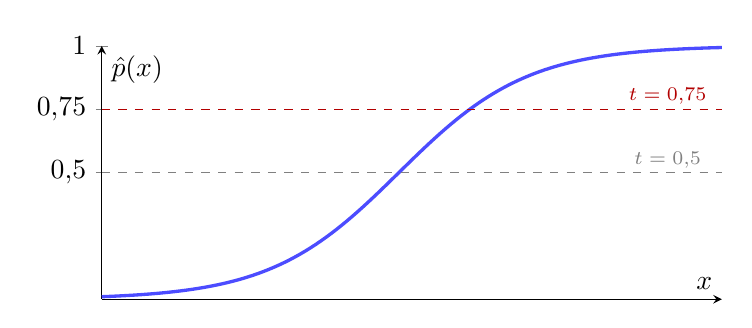
\begin{tikzpicture}
    \begin{axis}[
        width=0.78\textwidth,
        height=4.8cm,
        xmin=0, xmax=8,
        ymin=0, ymax=1,
        axis lines=middle,
        xlabel={$x$},
        ylabel={\(\hat p(x)\)},
        xtick=\empty,
        ytick={0,0.5,0.75,1},
        yticklabels={$0$,$0{,}5$,$0{,}75$,$1$},
        clip=false
    ]
        \addplot[
            very thick,
            blue!70,
            domain=0:8,
            samples=120
        ] {1/(1+exp(-(1.2*x-4.6)))};

        \addplot[dashed, gray] coordinates {(0,0.5) (8,0.5)};
        \addplot[dashed, red!70!black] coordinates {(0,0.75) (8,0.75)};

        \node[font=\scriptsize, gray] at (axis cs:7.3,0.55) {\(t=0{,}5\)};
        \node[font=\scriptsize, red!70!black] at (axis cs:7.3,0.80) {\(t=0{,}75\)};
    \end{axis}
\end{tikzpicture}
